\section{Detectors}\label{sec:detectors}

\subsection{Operating principle of an interferometric detector}\label{sec:principles}
All of the man-made detectors discussed in this section work on the principle of interferometry. Such detectors work by taking a beam of monochromatic light and splitting it into two beams travelling at some angle to each other. Each beam is passed in to a Fabry-P\'{e}rot cavity where it undergoes a number of round trips before being recombined to form an interference pattern. The ends of the cavity are, in the ideal case, freely floating test masses which move in response to a passing GW, this effect is measured by observing the changing interference pattern.

The response of a detector to an incident plane fronted GW depends upon the relative orientations of the detector and the incoming wave. Choose the origin of our coordinate system to be the beam-splitter of the interferometer and let $l_{1}^{i}$ and $l_{2}^{i}$ be unit 3-vectors pointing along the two arms. In the absence of noise the output of the detector is the difference in strain between the two arms \citep{MTW}
\begin{equation}\label{eq:hoftxx} h(t)=\frac{1}{2}h_{ij}\left( l_{1}^{i}l_{1}^{j}-l_{2}^{i}l_{2}^{j} \right)\; , \end{equation}
where $h_{ij}$ are the spatial components of the GW metric perturbation. Let $n^{i}$ be the unit 3-vector pointing towards the source of the GWs, with spherical polar angles $(\theta,\phi)$ relative to some axes fixed to the detector, also let $p^{i}$ and $q^{i}$ be unit vectors orthogonal to $n^{i}$. There remains a freedom in the coordinates described, a rotation of $p^{i}$ and $q^{i}$ through an angle $\psi$ about $n^{i}$. Define the basis tensors,
\begin{eqnarray}
H^{+}_{ij}&=p_{i}p_{j}-q_{i}q_{j} \nonumber \\
H^{\times}_{ij}&=p_{i}q_{j}+q_{i}p_{j} \; .
\end{eqnarray}
Consider a single frequency component of the incident GW, the strain induced by the incident GW may be written as
\begin{equation}\label{eq:hijxx} h_{ij}=A_{+}H^{+}_{ij}\cos\left(2\pi ft\right)+A_{\times}H^{\times}_{ij}\cos\left(2\pi ft+\Delta \phi\right) \; ,\end{equation}
where $A_{+}$ and $A_{\times}$ are the amplitudes of the two polarisation states. Combining (\ref{eq:hoftxx}) and (\ref{eq:hijxx}) allows the detector output to be written as
\begin{equation} h(t)=F^{+}(\theta,\phi,\psi)A_{+}\cos\left(2\pi ft\right)+F^{\times}(\theta,\phi,\psi)A_{\times}\cos\left(2\pi f t + \Delta\phi \right)\; , \end{equation}
where the response functions inherit their angular dependence from the choice of coordinates,
\begin{eqnarray}\label{eq:responsefuncs}
F^{+}(\theta,\phi,\psi)&=\frac{1}{2}H^{+}_{ij}\left(l_{1}^{i}l_{1}^{j}-l_{2}^{i}l_{2}^{j}\right) \nonumber \\
F^{\times}(\theta,\phi,\psi)&=\frac{1}{2}H^{\times}_{ij}\left(l_{1}^{i}l_{1}^{j}-l_{2}^{i}l_{2}^{j}\right) \; . 
\end{eqnarray}
The response function of a two-arm interferometric detector is quadrupolar, an example is plotted in figure \ref{fig:LIGO}.

\begin{figure}[h!]
 \centering
 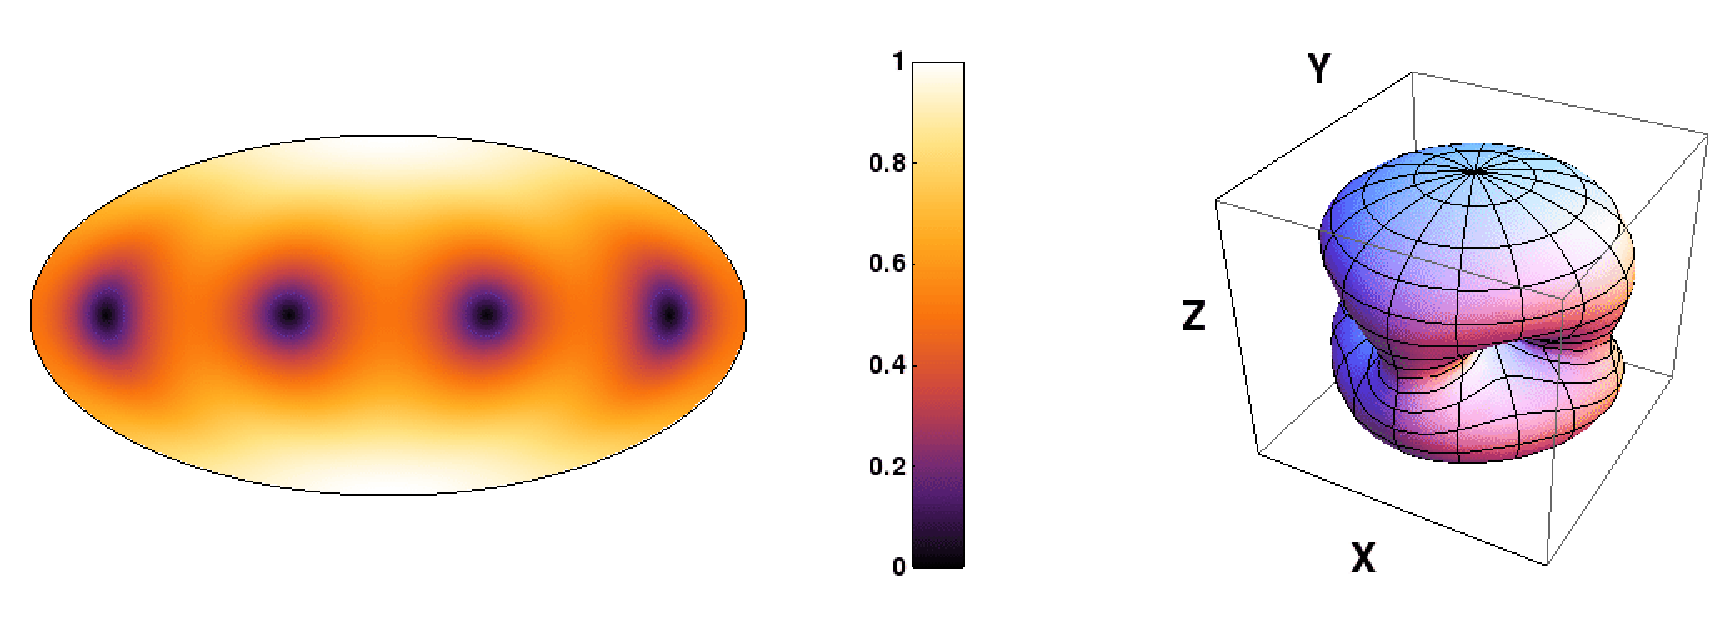
\includegraphics[trim=0cm 0cm 0cm 0cm, width=0.99\textwidth]{LIGO_detectorframe.pdf}
 \caption{The angular response function of an interferometric detector shown both as a surface plot and in an Aitoff-Hammer projection. The two detector arms lie in the $xy$ plane either side of one of the zeros in the response.}
 \label{fig:LIGO}
\end{figure}

Throughout this paper detector sensitivity refers to the polarisation and sky averaged sensitivity, $F$, where
\begin{equation}\label{eq:skyav} F^{2}=\int_{0}^{2\pi}\frac{\textrm{d}\psi}{2\pi}\; \int_{0}^{\pi}\int_{0}^{2\pi}\frac{\sin\theta\,\textrm{d}\theta\textrm{d}\phi}{4\pi}\;\left(\frac{F^{+}\left(\theta,\phi,\psi\right)^{2}+F^{\times}\left(\theta,\phi,\psi\right)^{2}}{2}\right)\; .\end{equation}
For a single $90\degree$ interferometer, such as LIGO (Laser Interferometer GW Observatory), the sky and polarisation averaged response is $F=\sqrt{1/5}\approx 0.447$.

A detector may consist of several interferometers. Let $F_{a}$ be the averaged response of the $a^{\textrm{th}}$ interferometer. The average response of the detector network is obtained by adding in quadrature,
\begin{equation} F_{\textrm{Total}}^{2}=\frac{1}{\left(\textrm{Number of interferometers}\right)}\sum_{x=1}^{N}F_{x}^{2} \; .\end{equation}

The averaging in (\ref{eq:skyav}) assumes a uniform distribution of polarisation angles $\psi$. This will be the case for a stochastic background, however for a non-inspiralling circular binary the polarisation will be a function of the two spherical polar angles ($\iota,\xi$) specifying the orientation of the binary's orbital angular momentum. Here $\iota$ is the polar angle between the orbital angular momentum and the line joining the source to the detector while $\xi$ is the azimuthal angle around the same line. In this case the correct average to characterise the detector sensitivity would be an an average over all four angles ($\theta,\phi,\iota,\xi$). If the binary is inspiralling then the polarisation will depend on still more parameters which need to be averaged over. These more complicated averages all have the property that they depend on both the detector and the source, hence they are unhelpful for our present purpose. In addition the different averages don't work out to be so different from each other; \cite{1993PhRvD..47.2198F} calculated the sensitivity for a detector with the LIGO geometry averaged over the four angles ($\theta,\phi,\iota,\xi$) as $\sqrt{4/25}=0.4$ times peak sensitivity, which should be compared with the value $\sqrt{1/5}\approx 0.447$ above. For the remainder of this paper the 3 angle average defined in (\ref{eq:skyav}) will be used.

\subsection{Ground based detectors}\label{sec:ground}
On Earth approximations to the free floating test masses described above are achieved by suspending the mass from a pendulum system with natural frequency much greater than that of the GW. The interferometric detectors listed in Table \ref{table:t} are all sensitive to GWs in the frequency range ${\cal{O}}(10-10^{3})\,\textrm{Hz}$. They all have multiple narrow lines in their sensitivity curves, which arise from noise sources in the instrument including resonances in the suspension system and electronic noise at multiples of $60\,\textrm{Hz}$: these have been removed in figures \ref{fig:hc}, \ref{fig:S} and \ref{fig:omega} for clarity. The detectors fall broadly into three categories: 1\textsuperscript{st} generation detectors, which have already operated; 2\textsuperscript{nd} generation detectors currently under construction; and 3\textsuperscript{rd} generation detectors at the planning stage. 

\begin{table}[h!]
\caption{\label{table:t} For the aVIRGO sensitivity curve an interpolation to the data published on \url{https://wwwcascina.virgo.infn.it/advirgo/} (2013) was used. For KAGRA (Kamioka Gravitational Wave Detector) an interpolation to the data for version D of the detector published on \url{http://gwcenter.icrr.u-tokyo.ac.jp/en/researcher/parameter} (2013) was used. For the remaining detectors analytic fits to the sensitivity curves due to \cite{Sathyaprakash} were used.}
\begin{indented}
\item[]\begin{tabular}{ l l l l l }
\br
{\bf Detector} & {\bf Country} & {\bf Arm length} & {\bf  Approximate date} & {\bf Generation} \\
\mr
  GEO600 	&	Germany 	& $600\,\textrm{m}$ 	& 2001-present 	   & 1$^{\textrm{st}}$\\
  TAMA300 	& 	Japan		& $300\,\textrm{m}$ 	& 1995-present     & 1$^{\textrm{st}}$\\
  iLIGO		&	US		& $4\,\textrm{km}$ 	& 2004-2010 	   & 1$^{\textrm{st}}$\\
  iVIRGO	& 	Italy		& $3\,\textrm{km}$ 	& 2007-2010 	   & 1$^{\textrm{st}}$\\
  aLIGO 	&	US		& $4\,\textrm{km}$ 	& \emph{est.} 2016 & 2$^{\textrm{nd}}$\\
  KAGRA		&	Japan		& $3\,\textrm{km}$ 	& \emph{est.} 2018 & 2$^{\textrm{nd}}$\\
  aVIRGO	&	Italy	 	& $3\,\textrm{km}$ 	& \emph{est.} 2017 & 2$^{\textrm{nd}}$\\
  ET (Einstein Telescope) &	Italy		& $10\,\textrm{km}$ 	& \emph{est.} 2025 & 3$^{\textrm{rd}}$\\
\br
\end{tabular}
\end{indented}
\end{table}


\subsection{Space based detectors}\label{sec:space}
Space based detectors work on similar principles to ground based detectors but with the test masses residing inside of independent, widely separated satellites. Space based detectors are sensitive to lower frequency GWs than their ground based counterparts, this is partly because space based detectors can have much longer arms and partly because they are unaffected by seismic noise which limits the low frequency performance of ground based detectors. 

The canonical design for a space based detector is LISA (Laser Interferometer Space Antenna), which would be sensitive to milli-Hz GWs. LISA would consist of three satellites flying in a triangular constellation with arms of length $5\times 10^{9}\,\textrm{m}$ in a $1\,\textrm{AU}$ orbit around the sun, trailing the Earth by $20\degree$. The laser arms in a LISA like detector are not a Fabry-P\'{e}rot cavity, the light only travels once along each arm. All of the sources discussed here lie within LISA's sensitivity reach. eLISA (evolved LISA) is a simpler version of LISA designed to probe the same frequency range, while proposals such as ALIA (Advanced Laser Interferometer Antenna), BBO (Big Bang Observer) and DECIGO (DECI-Hertz Interferometer GW Observatory) are designed to probe deci-Hz GWs.

\subsubsection{LISA and eLISA}
We use an analytic fit to the instrumental noise curve given by \cite{Sathyaprakash}. When observing individual sources with LISA there is an additional contribution to the noise from a background of unresolvable binaries. This is not included here as we consider the background as a source of GWs, see section \ref{sec:GB}. eLISA is a re-scoped version of the classic LISA mission, the main differences are shorter arms ($10^{9}\,\textrm{m}$ instead of $5\times 10^{9}\,\textrm{m}$), two laser arms instead of three and a different orbit (drifting away from Earth instead of $20\degree$ Earth trailing). The effect of these changes is a slightly reduced peak sensitivity and a shift to higher frequencies. We use an analytic fit to the instrumental noise curve given by \cite{Amaro-Seoane-et-al}.

\subsubsection{ALIA, DECIGO and BBO}
These missions are designed to probe the deci-Hz region of the GW spectrum, they are considerably more ambitious than the LISA or eLISA mission and their launches will be further into the future. For ALIA a simple analytic fit to the sensitivity curve is used, while for DECIGO and BBO fits to the sensitivity curves given by \cite{2011PhRvD..83d4011Y} are used.



\subsection{Pulsar timing arrays (PTAs)}\label{sec:PTAgeneralproperties}
PTAs can be thought of as naturally occurring interferometers with galactic scale arm lengths, hence they are sensitive to much lower frequencies than the detectors considered so far. Each pulsar is a very regular clock and the measured pulse arrival time (in practice, arrival times are corrected to arrival times at the solar-system  barycenter, SSB) can be compared against a prediction leaving a residual which includes the effects of passing GWs. Using an array of these pulsars spread across the sky allows us to correlate residuals between different pulsars and exploit the fact that the GWs influence all pulsars where as intrinsic pulsar noise clearly does not. The correlation between different pulsars depends only on their angular separation on the sky and has a distinctive shape, known as the Hellings and Downs curve \citep{HellingsDowns}, which we will now derive.

The redshift of the rate of arrival of pulses for a pulsar at a distance $L$ from Earth, in the direction of the unit spatial vector $\vec{p}$ induced by a GW travelling in the direction of the unit vector $\hat{\Omega}$ is given by \citep{anholm-2009}
\begin{equation}\label{eq:pulsarredshift} z(t,\hat{\Omega})=\frac{1}{2}\frac{\hat{p}^{j}\hat{p}^{i}} {1+\hat{\Omega}\cdot\hat{p}}\left(h_{ij}^{\textrm{Pulsar}}(t-L,\hat{\Omega} )-h_{ij}^{\textrm{Earth}}(t,\hat{\Omega} )\right)=\frac{1}{2}\frac{\hat{p}^{j}\hat{p}^{i}} {1+\hat{\Omega}\cdot\hat{p}}\Delta h_{ij}(t,\hat{\Omega})\; . \end{equation}
The redshift includes two terms, the pulsar term and the Earth term. The pulsar term is often neglected in PTA analysis as it can be considered as an extra noise term which averages to zero. The experimentally measured quantity is not the redshift but the timing residual, the two are related via
\begin{equation}\label{eq:restored}  R(t,\hat{\Omega})=\int_{0}^{t}\textrm{d}t'\;z(t',\hat{\Omega}) \; . \end{equation}
All of the pulsars, and the Earth, reside in the same metric perturbation field which may be expressed in terms of its Fourier transform
\begin{equation} h_{ij}(t,\hat{x})=\sum_{A=+,\times}\int\textrm{d}f\;\iint_{S_{2}}\textrm{d}\hat{\Omega}\; \tilde{h}_{A}(f,\hat{\Omega})e_{ij}^{A}(\hat{\Omega})e^{ 2\pi i f (t-\hat{\Omega}\cdot\vec{x}) } \; ,\end{equation}
where $e^{A}_{ij}(\hat{\Omega})$ is the $A$ polarisation basis tensor for direction $\hat{\Omega}$. Choosing the SSB as the origin of our coordinate system, so the pulsar is at position $L\hat{p}$, gives
\begin{equation}\label{eq:deltahij} \Delta h_{ij}(t,\hat{\Omega})=\sum_{A=+,\times}\int\textrm{d}f\; \tilde{h}_{A}(f,\hat{\Omega})e_{ij}^{A}(\hat{\Omega})e^{ 2\pi i f t }\left(e^{-2\pi\rmi fL (1+\hat{p}\cdot\hat{\Omega})}-1\right) \; . \end{equation}
From (\ref{eq:pulsarredshift}) and (\ref{eq:deltahij}) the Fourier transform of the redshift, $\tilde{z}(f,\hat{\Omega})$, may be read off as
\begin{equation}\label{eq:45} \tilde{z}(f,\hat{\Omega})=\left(e^{-2\pi\rmi fL (1+\hat{p}\cdot\hat{\Omega})}-1\right)\sum_{A=+,\times} \tilde{h}_{A}(f,\hat{\Omega})F^{A}(\hat{\Omega})\;, \textrm{where}\; F^{A}(\hat{\Omega})=\frac{e_{ij}^{A}(\hat{\Omega})\hat{p}^{j}\hat{p}^{i}} {2(1+\hat{\Omega}\cdot\hat{p})} \, .\end{equation}
The function $F^{A}(\hat{\Omega})$ may be regarded as the PTA equivalent of the detector response functions in (\ref{eq:responsefuncs}). The stochastic background of GWs is fully characterised by the one-sided power spectral density via the following expectation value
\begin{equation}\label{eq:stochback} \left<h_{A}^{*}(f,\hat{\Omega})h_{A'}(f',\hat{\Omega}')\right>=\frac{1}{2}S_{h}(f)\delta^{(2)}(\hat{\Omega},\hat{\Omega}')\delta_{AA'}\delta(f-f') \; ,\end{equation}
where $\delta^{(2)}(\hat{\Omega},\hat{\Omega}')$ is the delta function on the sphere. From (\ref{eq:stochback}) and (\ref{eq:45}) the expectation of the product of signals from two different pulsars in directions $\hat{p}_{1}$ and $\hat{p}_{2}$ may be evaluated
\begin{eqnarray} & \left<z_{1}(f)z_{2}^{*}(f')\right>=\frac{1}{2}S_{h}(f)\delta (f-f')\Gamma(f)\quad \textrm{where,} \\
& \Gamma(f)=\sum_{A=+,\times}\iint_{{\cal{S}}^{2}}\textrm{d}\hat{\Omega}\,\left(e^{2\pi\rmi fL_{1}(1+\hat{\Omega}\cdot\hat{p}_{1})}-1\right)\left(e^{-2\pi\rmi fL_{2}(1+\hat{\Omega}\cdot\hat{p}_{2})}-1\right)F_{1}^{A}(\hat{\Omega})F_{2}^{A}(\hat{\Omega}) \; . \nonumber\end{eqnarray}
The overlap function, $\Gamma(f)$, tends to a constant value in the limit that the distances to the pulsars are large compared to the wavelength of GWs, PTAs operate in this limit, so the overlap may be approximated as a constant 
\begin{equation} \Gamma(f)\approx\Gamma_{0}= \sum_{A=+,\times}\iint_{{\cal{S}}^{2}}\textrm{d}\hat{\Omega}\;F_{1}^{A}(\hat{\Omega})F_{2}^{A}(\hat{\Omega})\;.\end{equation}
Neglecting the exponential terms in the overlap is the frequency domain equivalent of neglecting the pulsar term in (\ref{eq:pulsarredshift}). The integral may be evaluated to give an expression depending only on the angle, $\theta$, between the two pulsars; this is the famous Hellings and Downs curve, see figure \ref{fig:HnD},
\begin{equation} \Gamma_{0}=\frac{1}{2}+\frac{3x}{2}\left(\log (x)-\frac{1}{6}\right) \quad \textrm{where}\quad x=\frac{1-\cos\theta}{2}\; .\end{equation}

\begin{figure}[h!]
 \centering
 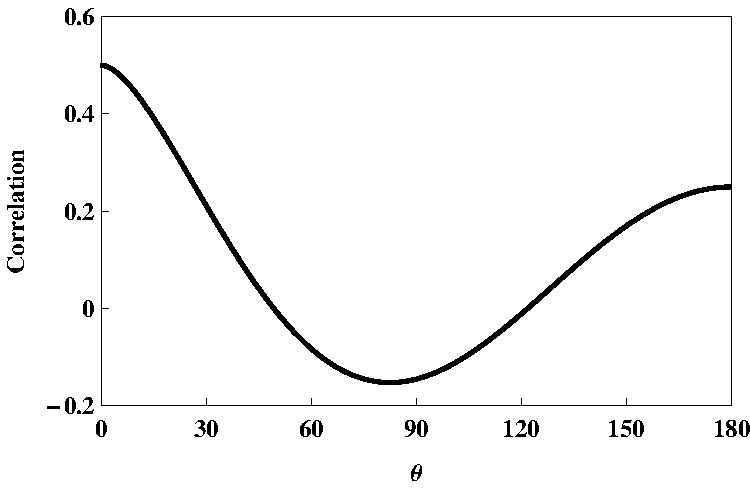
\includegraphics[trim=0cm 0cm 0cm 0cm, width=0.6\textwidth]{HnDcurve.pdf}
 \caption{The Hellings and Downs curve, the correlation between two pulsars seperated on the sky by an angle $\theta$.}
 \label{fig:HnD}
\end{figure}

The sensitivity bandwidth of a PTA is set by the sampling properties of the data set. If measurements are spaced in time by $\delta t$ and taken for a total length of time $T$ then the PTA is sensitive to frequencies in the range $(1/T)<f<(1/\delta t)$. The characteristic strain that the PTA is sensitive to scales linearly with $f$ in this range. This gives the wedge shaped curves plotted in figures \ref{fig:hc}, \ref{fig:S} and \ref{fig:omega}. The absolute value of the sensitivity is fixed by normalising to a calculated limit at a given frequency for each PTA. For a discussion of the sensitivities of PTA to both individual sources and stochastic background see \cite{MooreTaylorGair}.

There is a discrepancy between the treatment of PTA sensitivity curves here and the higher frequency detectors discussed in sections \ref{sec:ground} and \ref{sec:space}. When observing a long lived source, such as an inspiral, with a high frequency detector the convention was to define a \emph{characteristic} strain to satisfy (\ref{eq:hc}). Here the convention is to leave the strain untouched and instead adjust the PTA sensitivity curve with observation time, again to satisfy (\ref{eq:hc}). This discrepancy is an unfortunate result of the conventions in use by the different GW communities; however it is also natural given the sources under observation. When observing a transient source, such as a burst or inspiral, which changes within the lifetime of the detector it is natural to consider the detector as performing constantly while the signal changes. However when observing a monochromatic source or a stochastic background which is unchanging over the detector lifetime it is more natural to consider the source as being fixed and the sensitivity of the detector gradually improving. All that is required by the definition in (\ref{eq:hc}) is that the ratio $h_{c}(f)/h_{n}(f)$ is constant.



\subsubsection{EPTA/PPTA/NANOGrav}
The PTAs currently in operation are the EPTA (European Pulsar Timing Array), PPTA (Parkes Pulsar Timing Array, based in  Australia) and NANOGrav (North American Nanohertz Observatory for GWs). There are published limits on the amplitude of the stochastic background from all three detectors: currently the lowest is from the EPTA, \cite{Haasteren}. The EPTA curves in the figures show the  published limit based on an analysis of 5 pulsars over approximately 10 years.

\subsubsection{IPTA}
Combining the existing arrays would yield a single PTA using approximately 4 times as many pulsars pulsars. The IPTA curves plotted in the figures are based on 20 pulsars timed for twice as long as the current EPTA.

\subsubsection{SKA}
The sensitivity curve plotted in figures \ref{fig:hc}, \ref{fig:S} and \ref{fig:omega} for the SKA (Square Kilometer Array) assume a values of $\delta t^{2}_{\textrm{r.m.s.}}$ a factor of 10 better than current PTAs and 20 pulsars timed for twice as long as the current EPTA.

